%visualization of trade-off
\begin{frame}{Heat Vs. Complexity Trade-off}

    \begin{figure}
            \centering
            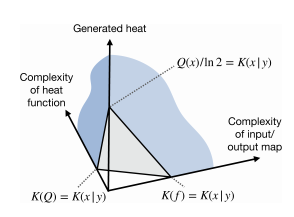
\includegraphics{HeatvsComplexity.png}
            \label{fig:HeatvsComplexity}
        \end{figure}
    
\end{frame}

%Bitstring Erasure Example
\begin{frame}{Heat VS. Complexity Trade-off}
    \begin{block}{Example: Erasing a Bitstring}
    \begin{equation*}
        Q(x)/\ln 2 + K(Q) + K(f) \ge K(x|y) + O(1)
    \end{equation*}
    \begin{itemize}
        \item Consider the an example where $f$ erases a long and incompressible bitstring $x$.
        \item $x\mapsto y$ comes with an intrinsic cost of $K(x|y) = K(x) \approx \ell(x)$
    \end{itemize}
    \end{block}
\end{frame}

%Pay cost by Generating Heat
\begin{frame}{Heat VS. Complexity Trade-off}
    \begin{block}{Generate a Lot of Heat}
    Take $f$ to be
    \begin{equation*}
        f(x') = `000...000' \:\forall x'
    \end{equation*}
    \begin{itemize}
        \item $f$ has low complexity
        \item Using dominating implementation, $Q(x)/\ln 2 = K(x|y) = K(x)\approx \ell(x)$
        \begin{itemize}
            \item Heat function has low complexity
            \item $x$ long and incompressible implies high heat generation
        \end{itemize}
    \end{itemize}
    \end{block}
\end{frame}

%Pay cost by having complex heat function Q
\begin{frame}{Heat Vs. Complexity Trade-off}
\begin{block}{Have a High Complexity Heat Function}
Can be shown that the following heat function satisfies conditions of Prop.1 for dominating realization of $f(x') = `000...000'$
\begin{equation*}
    Q(x') := \begin{cases} Q_\text{dom}(x') &x'\not\in \{x,`000...000'\}\\
    Q_\text{dom}(`000...000') &x' =x\\
    Q_\text{dom}(x) &x' = `000...000'\end{cases}
\end{equation*}
\begin{itemize}
    \item Generates little heat
    \item Low complexity $f$
    \item $x$ hard-coded into $Q$ implies high complexity heat function
\end{itemize}
\end{block}
\end{frame}

%pay cost by having high complexity mapping
\begin{frame}{Heat Vs. Complexity Trade-off}
\begin{block}{Have a High Complexity Mapping}
Consider the logically reversible map:
\begin{equation*}
    f(x') := \begin{cases} x' & x\not\in \{x,`000...000'\}\\
    `000...000' & x=x'\\
    x & x'= `000...000'\end{cases}
\end{equation*}
\begin{itemize}
    \item Logically reversible maps can be carried out with 0 heat generation
    \item 0 heat generation would imply minimally complex heat map
    \item $x$ hard-coded into $f$ implies high complexity mapping
\end{itemize}
\end{block}
\end{frame}
